\chapter{Statistical Mechanics - II}
\section{Thermodynamics of Magnetic System}
We consider a system of N dipoles with $J=\frac{1}{2}, $and suppose there is no interaction among the dipole. The dipole can be oriented in two direction and the corresponding energies are $\epsilon_i=-\mu_BH \quad\text{or} \quad\mu H$ when placed in magnetic field $H$.
$$\mathrm{Z}_{\mathrm{N}}(\mathrm{V}, \mathrm{T})=\left(\mathrm{e}^{\beta \mu H}+\mathrm{e}^{-\beta \mu H}\right) ^\mathrm{N}=\left[ 2\cosh(\beta\mu H)\right]^N $$
\textbf{Helmholtz Free Energy }
\begin{align*}
A&=-k_B T\ell nZ_N(V,T)=-k_BT \ell n (2\cosh(\beta\mu H))^N\\
\mathrm{A}&=-\mathrm{Nk}_{\mathrm{B}} \mathrm{T} \operatorname{\ell n} 2 \cosh (\beta\mu H)
\intertext{\textbf{Internal Energy (U):}}
\mathrm{U}&=-\mathrm{N} \mu H\tanh \frac{\mu H}{\mathrm{k}_{\mathrm{B}} \mathrm{T}}
\intertext{\textbf{Magnetisation (m):}}
M&=-\left(\frac{\partial A}{\partial H}\right)_{T}=N \mu \tanh \frac{\mu H}{k_{B} T} \\
\text{So}\quad U&=-M H
\end{align*}
\section{Ising Model}
Ising model was set up to investigate the bahaviour of substances whose molecules possess a magnetic moment.\\
eg: Ferromagnetic substances
$$E=-J \sum \sigma_{i} \sigma_{j}-\mu_{B}  \sum \sigma_{i}$$
\begin{align*}
E&\quad \rightarrow \text{ Total energy} \\
-J \sum \sigma_{i} \sigma_{j}&\quad \rightarrow  \text{Interaction energy}\\
-\mu_{B} H\sum \sigma_{i}&\quad  \rightarrow \text{Interaction energy energy asosiated with magnetic field H}\\
\sigma_{i}\text{ and } \sigma_{j} &\text { are ising spins }=\pm 1\\
\textbf{Partition Function}
\intertext{Energy due to nearest neighbour interaction,}
E_{\text {int. }}&=\left\{\begin{array}{l}
-J \quad \text { if } \sigma_{i}=\sigma_{j}=\pm1, \operatorname{deg}=2\\
+J\quad \text { if } \sigma_{i}=1 \text{ and }\quad \sigma_{j}=-1 \text{ or } \sigma_{i}=-1,\text{ and }  \sigma_{j}=+1, \operatorname{deg}=2
\end{array}\right.\\
Z_{int}=\sum g_{i} e^{-\beta \varepsilon_{i}}\\
&=2 e^{\beta J}+2 e^{-\beta J}\\
&=2.2(\cos h \beta J) \Rightarrow 2^{2}(\cosh \beta J)^{\prime}\\
\intertext{
Energy due to interaction with magnetic field, H}
E_{\text {H }}&=\left\{\begin{array}{l}
-\mu H, \sigma_i=+1\\
\mu H, \sigma_i=-1
\end{array}\right.\\
Z&=e^{-\beta \mu H}+e^{\beta \mu H}\\
Z_H&=2\cosh(\beta \mu H)\\
Z_N&=2^N\left[\cosh (\mu \beta H)^N \right] \\
Z_{Total}&=Z_{int}\times Z_H\\
&=2^N\cosh  (\beta J)^{N-1}\times2^N\cosh(\beta \mu H)^N
\end{align*}



\section{Harmonic Oscillator :}
\renewcommand*{\arraystretch}{2}
\begin{tabular}{|p{6cm}|p{6cm}|}
	\hline
	Classical Linear H.O&Quantum Linear H.O\\
	\hline
	$z_{1}=\frac{k_{B} T}{\hbar \omega}=\left(\frac{1}{\beta \hbar \omega}\right)$&$z_{1}=e^{-\beta \hbar \omega / 2}\left[\frac{1}{1-e^{-\beta \hbar \omega}}\right]$\\\hline
	$Z_{N}=\left(\frac{k_{B}}{\hbar \omega}\right)^{N}$&$Z_{N}=\left[2 \sinh \left(\frac{\beta \hbar \omega }{2}\right)^{-N}\right.$\\\hline
	$\langle u\rangle=N k_{B} T$&$\langle u\rangle=\frac{\hbar \omega}{2} N \coth \left(\frac{\beta \hbar \omega}{2}\right)$\\\hline
	$\langle P\rangle=0 \Rightarrow G=A$&$\langle P\rangle=0 \Rightarrow G=A$\\\hline
\end{tabular}
\section{Energy Fluctuation}
\begin{align*}
U&=\left\langle E_{i}\right\rangle=\sum E_{i} P_{i}\\
\frac{\partial U}{\partial \beta}&=\frac{\partial}{\partial \beta}\left\langle E_{i}\right\rangle=\langle E\rangle^{2}-\langle E\rangle^{2}\\
(\Delta E)^{2}&=-\frac{\partial U}{\partial \beta}=K T^{2} C_{V}
\end{align*}
\begin{tabular}{|p{3cm}|p{3cm}|p{3cm}|p{2cm}|p{3cm}|}
	\hline
	system&mean square energy&RMS energy&Relative mean square&Relative RMS\\\hline
	Non-Relative\newline Ideal gas&$\frac{3}{2} N K^{2} T^{2}$&$\sqrt{\frac{3 N}{2}} K T$& $\frac{2}{3 N}$&$\sqrt{\frac{2}{3N}}$\\\hline
	Classical \newline L.H.O&$N K^{2} T^{2}$&$\sqrt{N} K T$&$\frac{1}{N}$&$\sqrt{\frac{1}{N}}$\\\hline
	&$(D E)^{2}$&$(\Delta E)$&$\left(\frac{\Delta E}{\langle E i\rangle}\right)^{2}$&$\left(\frac{\Delta E}{\left\langle E_{i}\right\rangle}\right)$\\\hline
\end{tabular}


\section{Maxwell-Boltzmann Statistics}
Consider a system consisting of a large number of particles which are identical and distinguishable. Consider an ideal gas taken in a vessel of volume V. The particles (molecules) in the gas are in random motion, they move in all possible directions with all possible velocities, colliding with each other and with the walls of the vessel. The collisions are considered to be elastic. But during each collision the energy and momentum of each particle change. The change in momentum and energy is continuous, but total energy of the system remains constant.\\
\par Let $\mathrm{n}_{1}, \mathrm{n}_{2}, \mathrm{n}_{3}, \ldots . \mathrm{n}_{\mathrm{i}} \ldots$ be the number of particles in the energy levels $\epsilon_{1}, \in_{2}, \in_{3} \cdots \epsilon_{i} \cdots$. The total number of particles and total energy of the system are constants.
\begin{equation}
\text{So, }\mathrm{n}_{1}+\mathrm{n}_{2}+\mathrm{n}_{3}+\ldots .+\mathrm{n}_{\mathrm{i}}+\ldots=\sum \mathrm{n}_{\mathrm{i}}=\mathrm{n}=\mathrm{a}\text{ constant}
\end{equation}
\begin{equation}
\mathrm{n}_{1} \epsilon_{1}+\mathrm{n}_{2} \epsilon_{2}+\ldots .+\mathrm{n}_{\mathrm{i}} \epsilon_{\mathrm{i}}+\ldots .=\sum \mathrm{n}_{\mathrm{i}} \epsilon_{\mathrm{i}}=\mathrm{E}=\text { a constant }
\end{equation}
\par Let us consider a group of adjacent cells in the phase space. Such a group is called a zone of cells. The cells are of equal size. So the size of a zone is proportional to the number of cells in it. Let $g_{i}$ be the number of cells in a zone, then the probability of finding particle in the zone will be proportional to $\mathrm{g}_{\mathrm{i}}$ and is called a priori probability for the zone. It is also called the degeneracy of the $\mathrm{i}^{\text {th }}$ energy group having energy $\in_{\mathrm{i}} \cdot$\\
\par Consider any one of the particles having energy $E_{i}$. This particle can occupy $g_{i}$ cells in $g_{i}$ ways. So for $n_{i}$ particles there are gi ways for each particle. Hence the total number of ways in which $n_{i}$ particles can be arranged in $g_{i}$ cells is $\overline{g_{i}} \times g_{i} \times g_{i} \times \ldots(n$ times $)=\left(g_{j}\right)^{\text {ni }}$. The total number of particles $=n$. From $\mathrm{n}$ particles, $\mathrm{n}_{\mathrm{i}}$ particles for the $\mathrm{i}^{\text {th }}$ energy state can be selected ${ }^{n} \mathrm{Cn}_{\mathrm{i}}$ ways. So the number of different ways for the first group $={ }^{n} C_{n_{1}}\left(g_{1}\right)^{n_{1}}$. Since we have arranged $n_{1}$ particles the remaining\\\\
particles is $\left(n-n_{1}\right)$. So for the second group, $n_{2}$ particles are to be taken from $\left(n-n_{1}\right)$ particles and the number of ways it can be arranged is $={ }^{n-n_{1}} C_{n_{2}}\left(g_{2}\right)^{n_{2}}=\frac{\left(n-n_{1}\right) !}{n_{2} !\left(n-n_{1}-n_{2}\right)} \times\left(g_{2}\right)^{n_{2}}$ and so on. The thermodynamic probability $\Omega$ of distribution is equal to the total number of ways of distributing $n_{1}, n_{2}, n_{3} \ldots$ particles in the energy group $\varepsilon_{1}, \varepsilon_{2}$, $\varepsilon_{3} \ldots \ldots .$
\begin{align*}
\Omega&=\frac{n !\left(g_{1}\right)^{n_{1}} \xi}{\left(n_{1}\right) ! \cdot\left(n-n_{1}\right) !} \times \frac{\left(n-n_{1}\right) !\left(g_{2}\right)^{n_{2}}}{\left(n_{2}\right) ! \cdot\left(n-n_{1}-n_{2}\right) !} \times \ldots \ldots\\
&=\frac{n ! \cdot\left(g_{1}\right)^{n_{1}} \cdot\left(g_{2}\right)^{n_{2}} \cdot\left(g_{3}\right)^{n_{3}} \ldots .\left(g_{i}\right)^{n_{i}} \ldots \ldots}{\left(n_{1}\right) ! \cdot\left(n_{2}\right) ! \cdot\left(n_{3}\right) ! \ldots .\left(n_{i}\right) ! \ldots \ldots \ldots}\\
\Omega&=n ! \cdot \Pi \frac{\left(g_{i}\right)^{n_{1}}}{\left(n_{i}\right) !}
\intertext{Taking logarithm}
\log _{\mathrm{e}} \Omega &=\log _{\mathrm{e}} \mathrm{n} !+\sum_{\mathrm{i}}\left[\log _{\mathrm{e}}\left(g_{\mathrm{i}}\right)^{\mathrm{n}_{1}}-\log _{\mathrm{e}} \mathrm{n}_{\mathrm{i}} !\right] \\
&=\log _{\mathrm{e}} n !+\sum_{\mathrm{i}}\left[\mathrm{n}_{\mathrm{i}} \log _{\mathrm{e}} g_{\mathrm{i}}-\log _{\mathrm{e}} \mathrm{n}_{\mathrm{i}} ! !\right.\\
\text { According to }&\text{Stirling's approximation, } \log _{\mathrm{e}} \mathrm{x} !=\mathrm{x} \log _{\mathrm{e}} \mathrm{x}-\mathrm{x}\\
\text{So }\log _{e} \Omega&=n \log _{e} n-n+\sum_{i}\left[n_{i} \log _{e} g_{i}-n_{i} \log _{e} n_{i}+n_{i}\right]\\
&=n \log _{\mathrm{e}} \mathrm{n}+\sum_{\mathrm{i}}\left[n_{\mathrm{i}} \log _{\mathrm{e}} \mathrm{g}_{\mathrm{i}}-\mathrm{n}_{\mathrm{i}} \log _{\mathrm{e}} \mathrm{n}_{\mathrm{i}}\right] \quad\left[\because \Sigma \mathrm{n}_{\mathrm{i}}=\mathrm{n}\right]
\intertext{Differentiating equation}
\mathrm{d}\left(\log _{\mathrm{e}} \Omega\right)&=\sum_{\mathrm{i}}\left[\mathrm{dn}_{\mathrm{i}} \log _{\mathrm{e}} g_{\mathrm{i}}-\mathrm{dn}_{\mathrm{i}} \log _{\mathrm{e}} \mathrm{n}_{\mathrm{i}}-\mathrm{n}_{\mathrm{i}} \frac{1}{\mathrm{n}_{\mathrm{i}}} \mathrm{dn} \mathrm{n}_{\mathrm{i}}\right]\\
&=\sum_{i}\left(\log _{e} g_{i}-\log _{e} n_{i}\right) d n_{i}-\sum_{i} d n_{i}\\
&=\sum_{i}\left(\log _{e} g_{i}-\log _{e} n_{i}\right) d n_{i} \text {. Since } \Sigma n_{i}\\
&=n \text { is a }\text { constant. So } \Sigma d n_{1}=0 \text {. }\\
&=\sum_{i} \log \frac{g_{i}}{n_{i}} d n_{i}=-\sum_{i} \log \frac{n_{i}}{g_{i}} d n_{i}
\intertext{The condition for the most probable distribution is}
d \Omega&=0\\
d\left(\log _{e} \Omega\right)&=0
\intertext{From equation (6) we have,}
-\sum_{i} \log \frac{n_{i}}{g_{i}} d n_{i}&=0\\
\text { or } \quad \sum_{i} \log \frac{n_{i}}{g_{i}} d n_{i}&=0
\intertext{From equation (1) and (2), we have}
\sum_{i} d n_{i}&=0
\text{(as $\mathrm{n}$ is a constant)}\\
\text{and }\sum_{i} \epsilon_{i} d n_{i}&=0
\text{(as $\mathrm{E}$ is a constant)}
\intertext{Applying the Lagrange method of undetermined multipliers, i.e., multiplying equation (9) by $\alpha$ and equation (10) by $\beta$ and adding the result to equation (8) we get,}
\sum\left(\log \frac{n_{i}}{g_{i}}+\alpha+\beta \epsilon_{i}\right) d n_{i}&=0
\intertext{But $d n_{i} \neq 0$ as they are variable quantities.}
\text { So } \log _{\mathrm{e}} \frac{\mathrm{n}_{\mathrm{i}}}{\mathrm{g}_{\mathrm{i}}}+\alpha+\beta \epsilon_{\mathrm{i}}&=0\\
\log _{\mathrm{e}} \frac{\mathrm{n}_{\mathrm{i}}}{\mathrm{g}_{\mathrm{i}}} &=-\left(\alpha+\beta \epsilon_{\mathrm{i}}\right) \\
\frac{\mathrm{n}_{\mathrm{i}}}{\mathrm{g}_{\mathrm{i}}} &=\mathrm{e}^{-\left(\alpha+\beta \epsilon_{\mathrm{i}}\right)}\\
\mathbf{n}_{\mathbf{i}}&=\frac{\mathbf{g}_{\mathbf{i}}}{e^{\left(\alpha+\beta \epsilon_{i}\right)}}
\intertext{This is the equation for the most probable distribution according to Maxwell-Boltzmann statistics.}
\text { Let } e^{-\alpha}&=A \text {, another constant }\\
\text { Then, } n_{i}&=\frac{A g_{i}}{e^{\beta \epsilon_{i}}}=A g_{i} e^{-\beta \epsilon_{i}}
\end{align*}
\begin{note}
	Suppose the energy of the system has continuous values, in the range from $\in$ to $\in+\mathrm{d} \in$, the density of states $\mathrm{g}_{\mathrm{i}}$ can be replaced by $g(\in) d \in$ and $\epsilon_{i}$ by $\in$. The distribution law given by equation (13) can be written as, $n(\in) d \in=\frac{\operatorname{Ag}(\in) d \in}{e^{\beta \epsilon}}$
\end{note}













\section{Maxwell's formula for velocity distribution}
Maxwell-Boltzmann distribution law is
$$
n_{i}=A g_{i} \mathrm{e}^{-\beta \epsilon_{i}}
$$
When the system has continuous energy values, in the range from $E$ to $E+d E$, then $g_{i}$ is replaced by $g(\in) d \in$ and $\epsilon_{i}$ by $\varepsilon$.

Then the number of molecules $\mathrm{dN}$ with energy between $\in$ and $\varepsilon+d \varepsilon$ can be written as,
\begin{align*}
\mathrm{dN}&=A \mathrm{e}^{-\beta \varepsilon} g(\varepsilon) \mathrm{d} \varepsilon\\
\text{But }A&=\frac{N}{Z}, \beta=\frac{1}{k T}\\
\mathrm{dN}&=\frac{\mathrm{N}}{\mathrm{Z}} \mathrm{e}^{-\epsilon \mathrm{kT}} \mathrm{g}(\in) \mathrm{d} \in\\
\text { But from equation (30) } \mathrm{g}(\epsilon) \mathrm{d} \in&=\frac{2 \pi \mathrm{V}}{\mathrm{h}^{3}}(2 \mathrm{~m})^{3 / 2} \epsilon^{1 / 2} \mathrm{~d} \in
\intertext{Substituting in equation(48)}
\mathrm{dN}&=\frac{\mathrm{N}}{\mathrm{Z}} \mathrm{e}^{-\epsilon \mathrm{kT}} \times \frac{2 \pi \mathrm{V}}{\mathrm{h}^{3}}(2 \mathrm{~m})^{3 / 2} \epsilon^{1 / 2} \mathrm{~d} \in
\intertext{Substituting the value of z}
Z&=\frac{V}{h^{3}}(2 \pi k m T)^{3 / 2} \text { from equation }(33)\\
\mathrm{dN}&=\frac{\mathrm{N} \times \mathrm{h}^{3}}{\mathrm{~V}(2 \pi \mathrm{kmT})^{3 / 2}} \times \mathrm{e}^{-\epsilon \mathrm{kT}} \times \frac{2 \pi \mathrm{V}}{\mathrm{h}^{3}}(2 \mathrm{~m})^{3 / 2} \epsilon^{1 / 2} \mathrm{~d} \epsilon\\
\frac{d N}{d \in}&=\frac{2 \pi N}{(\pi k T)^{3 / 2}} \epsilon^{1 / 2} e^{-\epsilon / k T}
\intertext{This is the formula for the energy distribution of the molecules in an ideal gas.}
\intertext{The variation $(\mathrm{dN} / \mathrm{d} \varepsilon)$ with $\varepsilon$ is as shown in Fig. $4.12$ for two different temperature.}
\end{align*}
\begin{figure}[H]
	\centering
	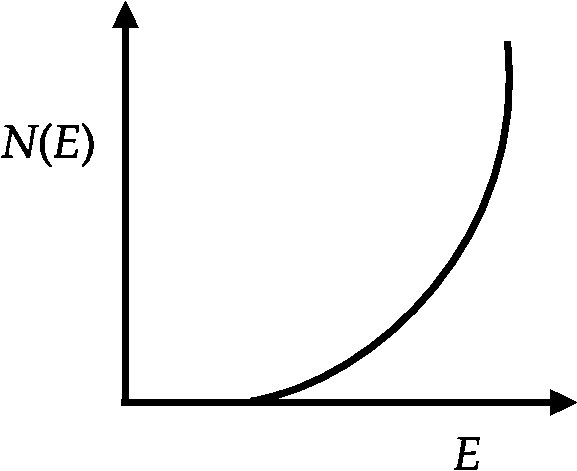
\includegraphics[height=5.5cm,width=6cm]{SM-01}
\end{figure}
\section{Velocity distribution formula}
\begin{align*}
\text { The energy of a molecule } \epsilon&=\frac{1}{2} m v^{2}, \frac{d \in}{d v}=m v
\intertext{Let $\mathrm{dN}$ be the number of molecules with speeds between $v$ and $v+d v$.}
\frac{\mathrm{dN}}{\mathrm{dv}}&=\frac{\mathrm{dN}}{\mathrm{d} \varepsilon} \cdot \frac{\mathrm{d} \varepsilon}{\mathrm{dv}}\\
\intertext{\text { Substituting equation (49) and }(50) \text { in (51). }}
\frac{d N}{d v}&=m v \times \frac{2 \pi N}{(\pi k T)^{3 / 2}}\left(\frac{1}{2} m v^{2}\right)^{1 / 2} e^{-m v^{2} / 2 k T}\\
\frac{\mathrm{dN}}{\mathrm{dv}}&=\frac{2 \mathrm{~N}}{\sqrt{2 \pi}}\left(\frac{\mathrm{m}}{\mathrm{kT}}\right)^{3 / 2} \mathrm{v}^{2} \mathrm{e}^{(-1 / 2) \mathrm{mv}^{2} / \mathrm{kT}}
\end{align*}
\par This is the Maxwells formula for the velocity distribution of the molecules in an ideal gas. This equation gives the number of molecules having a velocity between $v$ and $v+d v$ which does not depend on the direction of motion. The variation of $\mathrm{dN} / \mathrm{dv}$ with velocity $v$ is as shown in Fig. 4.13.\\
\begin{figure}[H]
	\centering
	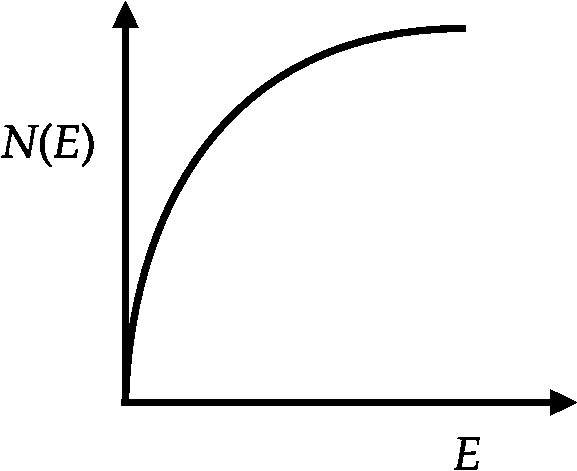
\includegraphics[height=4.5cm,width=6cm]{SM-02}
\end{figure}
\par The variation of $\mathrm{dN} / \mathrm{dv}$ with speed for two different temperatures $\left(\mathrm{T}_{2}>\mathrm{T}_{1}\right)$ as shown in Fig. 4.14. The higher the temperature the wider is the spread of the values of the speed.\\
From the graph the following conclusions are drawn.
\begin{enumerate}
	\item There is no molecule having zero speed.
	\item With increase in speed, the number of molecules in a given speed interval $\Delta \mathrm{v}$ increases upto a certain maximum value. The speed corresponding to the maximum number of molecules is called the most probable speed $v_{p}$ at that temperature.
	\item  When the speed increases beyond $v_{p}$, the number of molecules decreases exponentially towards zero. This means a molecule can have infinite speed according to classical statistics.
	\item With increase in temperature the value of $v_{p}$ increases and the range of speed also becomes greater. The graph becomes broader.
	\item The area under the graph is equal to the total number of molecules in the gas.
\end{enumerate}
\begin{figure}[H]
	\centering
	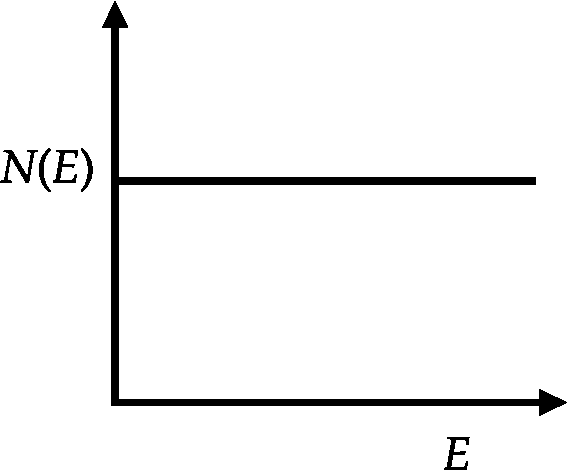
\includegraphics[height=5cm,width=5.5cm]{SM-03}
\end{figure}
\subsection{Most Probable Speed $\left(\mathbf{v}_{\mathrm{p}}\right)$}

The most probable speed $\left(v_{p}\right)$ of the molecules is that speed at which the number of molecules per unit range of speed is maximum.
$$
v_{p}=\sqrt{\frac{2 k T}{m}}
$$
\par where $T$ is the temperature of the gas, $k$ is the Boltzmann's constant and $m$ is the mass of the molecule.\\
\textbf{Average speed}
\par The arithmetic mean of the speeds of the molecules in the gas at a given temperature is called average speed $\overline{\mathbf{v}}$.
$$\bar{v}=\sqrt{\frac{8 k T}{\pi m}}$$
\subsection{Rms speed}
The root means square speed of a gas molecule is the square root of the mean of the squares of the speeds of the individual molecule. The rms speed $v_{r m s}$ is
\begin{align*}
\mathrm{v}_{\mathrm{rms}}&=\sqrt{\frac{3 \mathrm{kT}}{\mathrm{m}}}\\
\text { For an ideal gas, } &V_{p}<\bar{v}<V_{r m s}\\
\text { From the equations }&(53),(54) \text { and }(55) \text { we have }\\
\frac{v_{p}}{\sqrt{2}}&=\frac{\bar{v}}{\sqrt{8 / \pi}}=\frac{v_{\mathrm{rms}}}{\sqrt{3}}=\sqrt{\frac{\mathrm{kT}}{\mathrm{m}}}\\
\text { Also } \bar{v}&=\frac{2}{\sqrt{\pi}} v_{p} \text { and } v_{r m s}=\sqrt{\frac{3}{2}} v_{p} \ldots \ldots .
\end{align*}
\begin{exercise}
	Find the most probable, average and root mean square speeds of nitrogen molecule at $27^{0} \mathrm{C}$. Given the molar mass of $\mathrm{N}_{2}$ molecule $=2.8 \times 10^{-3} \mathrm{~kg} / \mathrm{mol}$, the gas constant $R=8.31 \mathrm{~J}$ $\mathrm{mol}^{-1} \mathrm{~K}^{-1}$.
\end{exercise}
\begin{answer}
	\begin{align*}
	\text { Most probable speed }&=v_{p}=\sqrt{\frac{2 \mathrm{kT}}{\mathrm{m}}}=\sqrt{\frac{2 \mathrm{RT}}{\mathrm{Nm}}}=\sqrt{\frac{2 \mathrm{RT}}{\mathrm{M}}}\\
	&=\sqrt{\frac{2 \times 8.31 \times 300}{28 \times 10^{-3}}}=4.22 \times 10^{2} \mathrm{~m} / \mathrm{s}
	\intertext{From equation
		$(56)$}
	\bar{v}=\frac{2}{\sqrt{\pi}} v_{p}&=\frac{2 \times 4.22 \times 10^{2}}{\sqrt{3.14}}=4.76 \times 10^{2} \mathrm{~m} / \mathrm{s}\\
	\mathrm{Rms} \text { speed }=\mathrm{v}_{\mathrm{rms}}&=\sqrt{\frac{3 \mathrm{kT}}{\mathrm{m}}}=\sqrt{\frac{3}{2}} \mathrm{v}_{\mathrm{p}}=\sqrt{\frac{3}{2}} \times 4.22 \times 10^{2}\\
	&=5.17 \times 10^{2} \mathrm{~m} / \mathrm{s}
	\end{align*}
\end{answer}
\begin{exercise}
	Calculate the most probable, the mean and the root mean square velocities of a molecule of a gas whose density under standard atmospheric pressure is $1 \mathrm{~kg} / \mathrm{m}^{3}$.
\end{exercise}
\begin{answer}
	The standard atmospheric pressure $=p$
	\begin{align*}
	&=1.013 \times 10^{5} \mathrm{~N} / \mathrm{m}^{2}\\
	\text { Density } \rho&=1 \mathrm{~kg} / \mathrm{m}^{3}\\
	\text { Most probable velocity } v_{p}&=\sqrt{\frac{2 k T}{m}}=\sqrt{\frac{2 P}{\rho}}\\
	&=\sqrt{\frac{2 \times 1.013 \times 10^{5}}{1}}=450 \mathrm{~m} / \mathrm{s}\\
	\text { The average speed } \bar{v}&=\frac{2}{\sqrt{\pi}} \times v_{p}=\frac{2 \times 450}{\sqrt{3.14}}=508 \mathrm{~m} / \mathrm{s}
	\end{align*}
\end{answer}
\section{Quantum Statistics}
\textbf{Introduction}\\
The main features of the quantum statistics are as follows:
\begin{enumerate}
	\item \textbf{ Bose-Einstein statistics}\\
In $B-E$ statistics, the particles are identical and indistinguishable. They have zero or integral spin. These particles are called Bosons. Bosons do not obey the Pauli's exclusion principle. Means there is no restriction to the number of Bosons staying together in the same quantum state. Examples of Bosons are $\alpha$-particle, $\pi$-mesons having spin zero $(0)$, photons and deutrons having spin one $(1)$.\\
\par The wave functions are symmetric. i.e., the sign of the wave function do not change on interchange of two bosons.
\item 
\textbf{ Fermi-Dirac statistics}\\
In $F-D$ statistics the particles are identical and indistinguishable, They have odd half-integral spin. (i.e., 1/2, 3/2, 5/2...) These particles are called Fermions. They obey Pauli's exclusion principle. This means only one fermion can occupy a particular quantum state of the system. Examples of fermions are electrons, protons, neutrons, $\mu$ meson, each having a spin half $(1 / 2)$ etc.
\end{enumerate}
\par The wave functions of a system of fermions are antisymmetric. i.e., The sign of the wave function changes on interchange of fermions.\\
\par Let us have a pictorial comparison of the three statistics. Consider two particles, say p and $q$, and two cells to be occupied.
\begin{enumerate}
	\item  \textbf{Classical statistics.} In this particles are identical, and distinguishable. So each or both of the particles can occupy any one of the two cells. Hence there are four possible arrangements for the distribution of two particles in two cells [See Fig. 4.15 (a)].\\
	\item  \textbf{Bose-Einstein statistics.} In this the particles are identical but indistinguishable. They do not obey Pauli's exclusion principle. So each cell may have any number of particles. Hence there are three possible arrangements [See Fig. $4.15$ (b)].
	\begin{figure}[H]
		\centering
		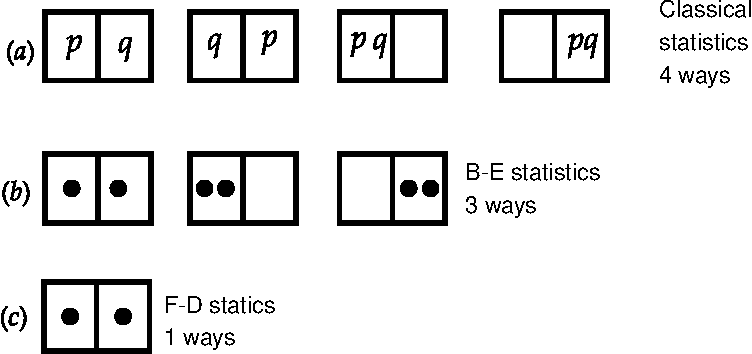
\includegraphics[height=3.7cm,width=9.5cm]{diagram-20220527-3-crop}
	\end{figure}
	\item  Fermi-Dirac statistics. In this, the particles are iđentical and indistinguishable. They obey Pauli's exclusion principle. So each cell will contain only one particle and hence only one arrangement is possible [See Fig. $4.15$ (c)].
\end{enumerate}
\subsection{Indistinguishability of identical particles}
The particles contained in a system can be classified into two type\\
(i) Distinguishable particle and \\(ii) Indistinguishable particle.
\begin{enumerate}[label=\roman*)]
	\item \textbf{ Distinguishable particles.} Particles which are dissimilar and can be distinguished from each other. There is no restrictions to the number of particles in any energy state. We do not consider the spin of the particles. These particles obey Maxwell-Boltzmann statistics and are called boltzons. We can apply the Maxwell-Boltzmann statistics to these particles provided the de Broglie wavelength of the particles is less than the mean distance between the particles.
	\item \textbf{Indistinguishable particles.} Particles which are similar and hence cannot be distinguished are called indistinguishable particles. The fundamental particles like electrons, protons, neutrons etc. have characteristic properties like charge, mass, spin, angular momentum etc. These parameters are the same for each of the particle. So they cannot be distinguished from each other and hence they are indistinguishable. We cannot apply classical statistics to them. The statistical mechanics applicable to indistinguishable particles is called quantum statistics. We have seen that there are two types of quantum statistics and correspondingly there are two types of particles, bosons and fermions.
\end{enumerate} 
\par The quantum statistics for particles having zero or integral multiple of $\mathrm{h} / 2 \pi$ spin was first established by s.N. Bose and hence those particles which obey B-E statistics are called bosons.\\
The quantum statistics for particles having an odd half-integral multiple of $\mathrm{h} / 2 \pi$ for their spin was first established by Fermi and hence those particles which obey F-D statistics are called Fermions.\\\\
When the position and spin coordinates of two particles are interchanged, if there is no physical way of measuring that a change has been made, then the particles are said to be indistinguishable.
In the case of classical mechanics, the particles, say molecules of a gas are distinguishable.\\\\
In the case of classical mechanics, the particles, say molecules of a gas are distinguishable. This is because eventhough the identical particles have the same physical properties they do not lose their individuality. This is because we can identify the particles by the continuity of their trajectories. But in the case of quantum mechanics, 
 due to uncertainty principle we cannot determine the position and momentum of the particle accurately and simultaneously. In quantum mechanics if path is determined accurately then there will be no definite value for the coordinates. So we cannot follow each of the smilar particle in a system containing a number of particles.
 More About Indistinguishability....
 To understand the indistinguishability of identical particles, let us consider a system containing $N$ identical particles occupying a volume V. In classical mechanics, we can determine $\mathrm{q}_{\mathrm{i}}$ and $\mathrm{p}_{i}$ simultaneously and accurately. But in quantum mechanics, we cannot, because of uncertainty principle.
 \subsection{More About Indistinguishability....}
 To understand the indistinguishability of identical particles, let us consider a system containing $\mathrm{N}$ identical particles occupying a volume V. In classical mechanics, we can determine $\mathrm{q}_{i}$ and $\mathrm{p}_{i}$ simultaneously and accurately. But in quantum mechanics, we cannot, because of uncertainty principle.\\\\
 There is a limit upto which we can apply classical mechanics. Let $\mathrm{p}_{\mathrm{av}}$ denote the average momentum of a molecule in the gas and let the intermolecular separation be $\mathrm{r}_{\mathrm{av}}$. Then classical method can be applied when $r_{a v} \cdot p_{a v}>>h$ where $h$ is the Planck's constant.
 \begin{align*}
 \text { De Broglie wavelength } \lambda&=\frac{h}{p}\\
 \text { Hence } \quad r_{a v} &\gg \frac{h}{p_{a v}}\\
 \text { or } r_{a v} &\gg \lambda_{a v}
 \end{align*}
 Under this condition the wave functions do not overlap and hence the particles can be distinguished.\\\\
 But when $r_{\text {av }} \ll \lambda_{\text {av }}$
 (2) then the wavefunction of one particle overlaps the other. Now the particle are indistinguishable.\\
 $r_{a v} \gg \lambda_{a v}$ gives the limit upto which classical mechanics can be applied. Using this classical limit we can obtain the conditions necessary for the application of classical statistics.\\\\
 Let us assume that each particle of the system occupy a very small cube of side $r_{\mathrm{av}}$. If $\mathrm{V}$ is the volume of $\mathrm{N}$ molecules then,
 \begin{align*}
 \mathrm{r}_{\mathrm{av}}^{3} N&=\mathrm{V}, \quad \mathrm{r}_{\mathrm{av}}=\left(\frac{V}{N}\right)^{1 / 3} \\
 \text { Let } \overline{\mathrm{E}}& \text { be the average energy at a temperature } \mathrm{T} \text {. }\\
 \text { Then } \overline{\mathrm{E}}&=\frac{\mathrm{p}_{\mathrm{av}}^{2}}{2 \mathrm{~m}}=\frac{3}{2} \mathrm{kT} \text { where } k \text { is the Boltzmann's constant and } \mathrm{m} \text { is the mass}\\
 \mathrm{p}_{\mathrm{av}}&=(3 \mathrm{mkT})^{12} \\
 \lambda_{\mathrm{av}}&=\frac{\mathrm{h}}{\mathrm{p}_{\mathrm{av}}}=\frac{\mathrm{h}}{(3 \mathrm{mkT})^{1 / 2}}\\
 \text { Substituting for } r_{a v} &\text { and } \lambda_{a v} \text { in equation (1) }\\
 &\left(\frac{V}{N}\right)^{1 / 3}>\frac{h}{(3 m k T)^{1 / 2}}
 \intertext{This equation shows that classical mechanics can be applied only when (i) $\mathrm{N}$ is small, (ii) $\mathrm{T}$ is high and (iii) $\mathrm{m}$ is not small.}
 \end{align*}
\section{ Bose-Einstein Distribution (B-E statistics)}
 B.E. statistics can be applied to particles which are identical and indistinguishable. The spin angular momentum of these particle is zero or integral multiple of $\mathrm{h} / 2 \pi$. These particles are called Bosons and they do not obey Pauli's exclusion principle. So there is no restriction to the number of bosons staying together in the any quantum state or phase cell. It is assumed that the sum of energies of all the particles in various quantum states is equal to the total energy of the system and is a constant. It is also assumed that the number of phase cells is comparable to the number of particles in the system. 1.e. $\mathrm{n}_{\mathrm{i}} / \mathrm{g}_{\mathrm{i}}=1$.\\\\
 Consider an isolated system consisting of weakly interacting particles, called bosons. Let the total number of particles in the system be $\mathrm{n}$ and has a volume $\mathrm{V}$. The system is assumed to be in equilibrium at a temperature $\mathrm{T}$ and its total energy is $\mathrm{E}$, which is a constant. Each particle in the system has a particular momentum and definite energy and can be represented by a point in the phase cell. We have to find maximum probable distribution of the particles in the phase space For this the phase space is divided into a large number of quantum\\
 groups or energy levels. These groups are again divided into phase cells of volume $h^{3}$ each.\\\\
 Let $\mathrm{n}_{1}, \mathrm{n}_{2}, \mathrm{n}_{3} \ldots \mathrm{n}_{\mathrm{i}} \ldots$ be the number of particles in groups whose approximate constant energies are $\epsilon_{1}, \in_{2}, \in_{3} \ldots \epsilon_{i} \ldots .$ respectively. The number of particles $n_{1}, n_{2} \ldots$ are called the occupation numbers of the levels. The number of phases cells $g_{i}$ in an energy level $\epsilon_{i}$ of the $i$ th level is called the degeneracies. The degeneracy of the energy levels $\epsilon_{1}, \epsilon_{2} \ldots$ are $g_{1}, g_{2} \ldots$ The degeneracy is also called the statistical weight of the $\mathrm{i}^{\text {th }}$ level.
 \begin{align*}
 \text { The total number of particles, }\\
 \mathrm{n}_{1}+\mathrm{n}_{2}+\mathrm{n}_{3}+\ldots .+\mathrm{n}_{\mathrm{i}}+\ldots&=\sum \mathrm{n}_{\mathrm{i}}=\mathrm{N} \text { is a constant. }\\
 \text { The total energy of the system, }\\
 \mathrm{n}_{1} \epsilon_{1}+\mathrm{n}_{2} \epsilon_{2}+\ldots .+\mathrm{n}_{\mathrm{i}} \epsilon_{\mathrm{i}}+\ldots&=\sum \mathrm{n}_{\mathrm{i}} \epsilon_{\mathrm{i}}=\mathrm{E} \text { is a constant }
 \end{align*}
 We have to find how $\mathrm{n}_{\mathrm{i}}$ indistinguishable particles are distributed among $\mathrm{g}_{\mathrm{i}}$ distinguishable levels. (remembering that there is no restriction in the number of particles that can occupy any one level). For this $\left(\mathrm{g}_{\mathrm{i}}-1\right)$ partitions are necessary. Thus $\mathrm{n}_{\mathrm{i}}$ particles are to be arranged in a row and distributed among $g_{i}$ quantum states with $\left(g_{\mathrm{i}}-1\right)$ partitionsin between. Then the total number of possible arrangements of particles and partitions is equal to the total number of permutations of $\left(n_{i}+g_{i}-1\right)$ particles in a row. Hence the total number of possible ways of arranging $\mathrm{n}_{\mathrm{i}}$ particles with $\left(\mathrm{g}_{\mathrm{i}}-1\right)$ partitions $=\left(\mathrm{n}_{\mathrm{i}}+\mathrm{g}_{\mathrm{i}}-1\right)$ !. In each of these arrangements the number of permutations of $n_{i}$ particles among themselves is $n_{i} !$ and that of $\left(g_{i}-1\right)$ partitions among themselves is $\left(g_{i}-1\right) !$. But the particles and partitions are identical and indistinguishable. So these permutations would not give any independent arrangements. Hence the number of independent permutations of $n_{i}$ particles among $g_{i}$ states is given by
 $$\omega_{i}=\frac{\left(n_{i}+g_{i}-1\right) !}{n_{i} !\left(g_{i}-1\right) !}$$
We can derive similar equations for other energy groups also. Hence the total number $W$ of independent ways of arranging $n$ particles in various quantum states is given by
\begin{align*}
\mathrm{W} \quad&=\omega_{1} \times \omega_{2} \times \omega_{3} \times \ldots .\\
&=\frac{\left(n_{1}+g_{1}-1\right) !}{n_{1} !\left(g_{1}-1\right) !} \times \frac{\left(n_{2}+g_{2}-1\right) !}{n_{2} !\left(g_{2}-1\right) !} \times \ldots \ldots\\
&=\prod_{i} \frac{\left(n_{i}+g_{i}-1\right) !}{n_{i} !\left(g_{i}-1\right) !}
\end{align*}
This equation represents the thermodynamic probability of the given distribution. The most probable distribution can be obtained by finding the maximum value of $\log _{\mathrm{e}} \mathrm{W}$. But $\mathrm{n}_{\mathrm{i}}$ and $\mathrm{g}_{\mathrm{i}}$ are very large and hence one $(1)$ is neglected.
\begin{align*}
W&=\prod_{i} \frac{\left(n_{i}+g_{i}\right) !}{n_{i} ! g_{i} !}\\
\text { Taking logarithm, }\\
\log _{\mathrm{e}} \mathrm{W}&=\sum_{i} \log \left(n_{\mathrm{i}}+g_{\mathrm{i}}\right) !-\log n_{\mathrm{i}} !-\log g_{\mathrm{i}} !\\
\text { Applying Stirling's formula, } \log x !&=x \log _{e} x-x \text {, we get }\\
\log _{e} W&=\sum_{i}\left(n_{i}+g_{i}\right) \log \left(n_{i}+g_{i}\right)-\left(n_{i}+g_{i}\right)-n_{i} \log n_{i}+n_{i}-g_{i} \log g_{i}+g_{i}\\
\log _{e} W&=\sum_{i}\left[\left(n_{i}+g_{i}\right) \log \left(n_{i}+g_{i}\right)-n_{i} \log n_{i}-g_{i} \log g_{i}\right]\\
\text { The maximum value of } W &\text { is obtained by taking } d\left(\log _{e} W\right)=0
\intertext{ Differentiating }\\
d\left(\log _{e} W\right)&=\sum_{i}\left[d n_{i} \times \log \left(n_{i}+g_{i}\right)+\left(n_{i}+g_{i}\right) \times \frac{1}{\left(n_{i}+g_{i}\right)} \times d n_{i}\right.\\
&\left.-d n_{i} \times \log n_{i}-n_{i} \times \frac{1}{n_{i}} \times d n_{i}-0\right]\\
0&=\sum_{i}\left[\log _{e}\left(n_{i}+g_{i}\right)-\log _{e} n_{i}\right] d n_{i} \quad \text { or } \\
\sum_{i}&\left[\log _{e} n_{i}-\log _{e}\left(n_{i}+g_{i}\right) d n_{i}=0\right.\\
\sum_{i} \log _{e}&\left(\frac{n_{i}}{n_{i}+g_{i}}\right) d n_{i}=0\\
\text { The total number }&\text{of particles in the system is a constant. }\\
\sum_{i} n_{i}&=n=a \text { constant }\\
\sum_{i} \varepsilon_{i} d n_{i}&=0
\intertext{Equation 5, 6, 7 are independent of each other, but in the equilibrium state they must be satisfied simultaneously.
	Lagrange's method of undetermined multipliers is used to get a common solution. Multiplying equation $(6)$ by $(\alpha)$, and equation (7) by (B) and adding the result to equation (5) we get.}
\sum_{i}\left[\log _{e}\left(\frac{n_{i}}{n_{i}+g_{i}}\right)+\alpha+\beta \varepsilon_{i}\right] &d n_{i}=0
\intertext{But $\mathrm{dn}_{\mathrm{i}}$ is a variable quantity and is not zero. So the coefficient of $\mathrm{dn}_{\mathrm{i}}$ must be zero.}
\log _{\mathrm{e}}\left(\frac{\mathrm{n}_{\mathrm{i}}}{\mathrm{n}_{\mathrm{i}}+\mathrm{g}_{\mathrm{i}}}\right)+\alpha+\beta \varepsilon_{\mathrm{i}}&=0 ; \log _{\mathrm{e}}\left(\frac{\mathrm{n}_{\mathrm{i}}}{\mathrm{n}_{\mathrm{i}}+\mathrm{g}_{\mathrm{i}}}\right)=-\left(\alpha+\beta \varepsilon_{\mathrm{i}}\right) \\
&\left(\frac{\mathrm{n}_{\mathrm{i}}}{\mathrm{n}_{\mathrm{i}}+\mathrm{g}_{\mathrm{i}}}\right)=\mathrm{e}^{-\left(\alpha+\beta \varepsilon_{\mathrm{i}}\right)} \\
&\left(\frac{\mathrm{n}_{\mathrm{i}}+\mathrm{g}_{\mathrm{i}}}{\mathrm{n}_{\mathrm{i}}}\right)=\mathrm{e}^{+\left(\alpha+\beta \varepsilon_{\mathrm{i}}\right)} \\
&1+\frac{\mathrm{g}_{\mathrm{i}}}{\mathrm{n}_{\mathrm{i}}}=\mathrm{e}^{\left(\alpha+\beta \varepsilon_{\mathrm{i}}\right)} \\
&\frac{\mathrm{g}_{\mathrm{i}}}{\mathrm{n}_{\mathrm{i}}}=\mathrm{e}^{\left(\alpha+\beta \varepsilon_{\mathrm{i}}\right)}-1\\
n_{i}&=\frac{g_{i}}{e^{\left(\alpha+\beta \varepsilon_{i}\right)}-1}
\intertext{This equation represents the most probable distribution of the particles among various energy levels of system, which obey BoseEinstein statistics.}
\end{align*}
\section{\text { Bose-Einstein Energy distribution function }}
The energy distribution function $f\left(\varepsilon_{\mathrm{i}}\right)$ is the average number of particles per quantum state in the energy level $\varepsilon_{i}$.
\begin{align*}
\frac{n_{i}}{g_{i}}&=\frac{1}{e^{\left(\alpha+\beta \varepsilon_{i}\right)}-1}\\
\text { For energy } &E \text {, equation (9) can be written as }\\
F(E)&=\frac{1}{e^{\left(\alpha+\beta E_{i}\right)}-1}
\end{align*}
\section{Fermi-Dirac Distribution (F-D statistics)}
In F-D statistics the particles are identical and indistinguishable. The spin angular momentum of these particles is odd half-integral multiple of $h / 2 \pi$ [i.e., $(1 / 2) \mathrm{h} / 2 \pi,(3 / 2) \mathrm{h} / 2 \pi \ldots \ldots]$. These particles are called Fermions. They obey Pauli's exclusion principle. This means only one fermion can occupy a particular quantum state of the system. Hence the degeneracy $g_{j}$ of an energy level must be larger than the number of particles to be distributed (i.e., $g_{i}>n_{i}$ ).\\\\
Consider an isolated system consisting of weakly interacting particles called fermions. Let the total number of particles in the system be $n$ and has a volume $\mathrm{V}$. The system is assumed to be in equilibrium at a particular temperature $T$ and its total energy $E$, which is a constant. The phase space is divided into a large number of quantum energy states. Let the energies of the states $1,2,3 \ldots .$ be $\in_{1}, \in_{2}, \in_{3} \ldots$. Each energy level consists of a number of phase cells. Let $g_{i}$ be the cells in the $i^{\text {th }}$ quantum state and $g_{i}$ is called the degeneracy of the $i^{\text {th }}$ level. It is assumed that $\mathrm{n}_{\mathrm{i}} \ll \mathrm{g}_{\mathrm{i}}$. This means that the $\mathrm{n}_{\mathrm{i}}$ value for a given distribution cannot be greater than the corresponding value of $g_{i}$.\\\\
Let the number of particles for the energy level $\epsilon_{\mathrm{i}}$ be $\mathrm{n}_{\mathrm{i}}$. Out of $\mathrm{g}_{\mathrm{i}}$ cells, $n_{i}$ cells will be filled with $n_{i}$ particles and $\left(g_{i}-n_{i}\right)$ cell be unfilled. The first particle can be placed in any one of the available $g_{i}$ states. This means we can distribute the first particle in $\mathrm{g}_{\mathrm{i}}$ different ways. Similarly the second particle can be arranged in $\left(g_{i}-1\right)$ different ways and so on. Hence the total number of different ways of arranging $\mathbf{n}_{i}$ particles among the $g_{\mathrm{i}}$ states with $\epsilon_{\mathrm{i}}$ energy levels,
\begin{align*}
=g_{i}\left(g_{i}-1\right)\left(g_{i}-2\right) \ldots \ldots \ldots\left[g_{i}-\left(n_{i}-1\right)\right]\\
&=\frac{g_{i} !}{\left(g_{i}-n_{i}\right) !}
\end{align*}
The particles are indistinguishable. So if $n_{i}$ particles are rearranged into different states occupied by them in the energy level $\epsilon_{i}$ it will not make any difference. So the total number of ways in which $n_{1}$ particles can be arranged in $g_{i}$ cells is,
$$\omega_{i}=\frac{g_{i} !}{n_{i} !\left(g_{i}-n_{i}\right) !}$$
We can derive similar equations for other energy states. Hence the total number of different and distinguishable ways $\mathrm{W}$ of distributing $n_{1}, n_{2}, n_{3} \ldots$. among the various energy levels $\epsilon_{1}, \epsilon_{2}, \in_{3} \ldots$ is obtained by multiplying the various expressions.
\begin{align*}
\mathrm{W}&=\frac{\mathrm{g}_{1} !}{\mathrm{n}_{1} !\left(\mathrm{g}_{1}-\mathrm{n}_{1}\right) !} \times \frac{\mathrm{g}_{2} !}{\mathrm{n}_{2} !\left(\mathrm{g}_{2}-\mathrm{n}_{2}\right) !} \times \frac{\mathrm{g}_{3} !}{\mathrm{n}_{3} !\left(\mathrm{g}_{3}-\mathrm{n}_{3}\right) !} \times \ldots\\
\mathrm{W}&=\prod \frac{\mathrm{g}_{\mathrm{i}} !}{\mathrm{n}_{\mathrm{i}} !\left(\mathrm{g}_{\mathrm{i}}-\mathrm{n}_{\mathrm{i}}\right) !}
\intertext{ The most probable distribution can be found out by evaluating the maximum value of $\log _{\mathrm{e}} \mathrm{W}$.}
\log _{e} W&=\sum_{i}\left[\log _{e} g_{i} !-\log n_{i} !-\log _{e}\left(g_{i}-n_{i}\right) !\right]\\
\text { Using Stirling's approximation, } &\log _{e} x !=x \log _{e} x-x\\
\log _{e} W&=\sum_{i}\left[g_{i} \log _{e} g_{i}-g_{i}-n_{i} \log _{e} n_{i}+n_{i}-\left(g_{i}-n_{i}\right) \log _{e}\left(g_{i}-n_{i}\right)\right.+g_{i}-n_{i} \mid\\
\log _{e} w&=\sum_{i}\left[g_{i} \log _{e} g_{i}-n_{i} \log _{e} n_{i}-\left(g_{i}-n_{i}\right) \log _{e}\left(g_{i}-n_{i}\right)\right] \ldots
\intertext{Differentiating equation (3). (remember $g_i$ is a constant)}
d\left(\log _{e} w\right)&=\sum_{i}-d n_{i} \log _{e} n_{i}-n_{i} \times \frac{1}{n_{i}} d n_{i}-\left(-d n_{i}\right) \log _{e}\left(g_{i}-n_{i}\right)-\\
&-\left(g_{i}-n_{i}\right) \times \frac{1}{\left(g_{i}-n_{i}\right)} \times\left(-d n_{i}\right)\\
&=\sum_{i}\left[-\log _{e} n_{i}+\log _{e}\left(g_{i}-\dot{n}_{i}\right)\right] d n_{i}\\
&=-\sum_{i} \log \frac{n_{i}}{\left(g_{i}-n_{i}\right)} d n_{i}\\
\text { To obtain the maximum value of } &W, d\left(\log _{e} W\right)=0\\
\sum_{i} &\log \frac{n_{i}}{\left(g_{i}-n_{i}\right)} d n_{i}=0\\
\text{ The total number of }&\text{particles in the system is a constant. }\\
\sum_{i} n_{i}&=n=a \text { constant. } \\
\sum_{i} d n_{i}&=0 \quad \ldots \ldots \ldots \ldots .(5)\\
\text { The total energy }&\text{of the system is a constant. }\\
\sum_{i} n_{i} \varepsilon_{i}&=\mathrm{E}=\text { a constant. } \\
\sum_{i} \varepsilon_{i} \mathrm{dn} n_{\mathrm{i}}&=0 \ldots \ldots \ldots \ldots(6)\\
\text{Multiplying equation(5)}&\text{ by $\alpha,(6)$ by $\beta$ and adding to equation (4)}\\
\sum_{i}\left[\log \left(\frac{n_{i}}{g_{i}-n_{i}}\right)+\alpha+\beta \varepsilon_{i}\right]& d n_{i}=0\\
\log \left(\frac{n_{i}}{g_{i}-n_{i}}\right)&=-\alpha-\beta \varepsilon_{i} \\
\frac{n_{i}}{g_{i}-n_{i}}&=e^{-\alpha-\beta \varepsilon_{i}} \\
\frac{g_{i}-n_{i}}{n_{i}}&=e^{+\alpha+\beta \varepsilon_{i}} \\
\frac{g_{i}}{n_{i}}-\frac{n_{i}}{n_{i}}&=e^{\alpha+\beta \varepsilon_{i}} \\
\frac{g_{i}}{n_{i}}&=e^{\alpha+\beta \varepsilon_{i}}+1\\
n_{i}&=\frac{g_{i}}{e^{\alpha+\beta \varepsilon_{i}}+1}
\intertext{Equation (7) represents the Fermi-Dirac distribution law. For a system consisting of fermions in statistical equilibrium, $\beta=\frac{1}{k T}$}
n_{i}&=\frac{g_{i}}{e^{\left(\alpha+\varepsilon_{i} / k T\right)}+1}
\intertext{In most cases $\alpha$ is negative and equal to $-\mathrm{E}_{\mathrm{F}} / \mathrm{kT}$, where $\mathrm{E}_{\mathrm{F}}$ is the fermi energy of the system and $\mathrm{k}$ is the Boltzmann's constant.}
n_{i}&=\frac{g_{i}}{e^{\left(-E_{F}+\varepsilon_{i}\right) / k T}+1}=\frac{g_{i}}{e^{\left(\varepsilon_{i}-E_{F}\right) / k T}+1}
\end{align*}
\section{Fermi-Dirac Distribution Function}
The Fermi-Dirac distribution function $f\left(\epsilon_{1}\right)$ is the ratio of the number of quantum state $(n, j)$ of energy $E_{j}$ occupied by the electrons to total number of quantum states avalable in the energy level $E_{i^{*}}$
$$
f\left(\epsilon_{i}\right)=\frac{n_{i}}{g_{i}}=\frac{1}{e^{\left(\epsilon_{1}-E_{F}\right) k T}+1}
$$
For any energy $E$, this equation can be written as,
$$
f(E)=\frac{1}{e^{(E-E F) / k T}+1}
$$
\begin{exercise}
 In how many ways can 2 particles be distributed in 5 states if the particles are indistinguishable and follow BoseEinstein statistics?
 \end{exercise}
\begin{answer}
	\begin{align*}
	\text { Given } \mathrm{n}_{\mathrm{i}}&=2 \text { and } \mathrm{g}_{\mathrm{i}}=5\\
	\omega_{i} &=\frac{\left(n_{i}+g_{i}-1\right) !}{n_{1} !\left(g_{i}-1\right) !}=\frac{(2+5-1) !}{2 !(5-1) !} \\
	&=\frac{6 !}{2 ! 4 !}=\frac{1 \times 2 \times 3 \times 4 \times 5 \times 6}{1 \times 2 \times 1 \times 2 \times 3 \times 4}=15
	\end{align*}
\end{answer}
\begin{exercise}
What is the number of possible arrangements for the distribution of 7 bosons in 4 cells of equal probability?
\end{exercise}
\begin{answer}
	\begin{align*}
 n_{i}&=7, g_{i}=4\\
	\omega_{i}&=\frac{\left(n_{i}+g_{i}-1\right) !}{n_{1} !\left(g_{i}-1\right) !}=\frac{(7+4-1) !}{7 !(4-1) !}\\
	&=\frac{10 !}{7 ! 3 !}=\frac{8 \times 9 \times 10}{1 \times 2 \times 3}+=120
	\end{align*}
\end{answer}
\renewcommand*{\arraystretch}{2}
\begin{tabular}{|p{5.5cm}|p{5.5cm}|p{5.5cm}|}
	\hline
\textbf{	Maxwell-Boltzmann}&\textbf{Fermi-Dirac}&\textbf{Bose-Einstein}\\\hline
	1. Particles are distinguishable.&1. Particles are indistinguishable.&1. Particles are distinguishable.\\
	2. Only particles are taken into consideration& 2. Only quantum states are taken into consideration& 2. Only quantum states are taken into consideration\\
	3. There is no restriction on the number of particles in a given state.&3. There is restriction on the number of particles in a given quantum state.&3. There is no restriction of particles in a given quantum state.\\
	4. Volume of the state in six dimensional space is not known&4. Phase space is known $V=h^3$&4. Phase space is known $V=h^3$\\
	5. Number of distinguishable ways are given by\newline$P \stackrel{n !}{=} \prod_{i}^{N} \frac{g_{i}^{n_{i}}}{n_{i} !}$&5. Number of distinguishable ways are given by\newline$P=\prod_{i} \frac{g_{i} !}{\left.n_{i} !\left(g_{i}-n_{1}\right)\right\}}$&5.  Number of distinguishable ways are given \newline$P=\prod_{i} \frac{g_{i} !}{\left.n_{i} !\left(g_{i}-n_{1}\right)\right\}}$\\
	6. Maximum probability distribution $x \frac{1}{e^{\left(\alpha+\beta \epsilon_{i}\right)}}$.&6. Maximum probability distribution\newline$\infty\frac{1}{\left[e^{\left(\alpha+\beta \epsilon_{i}\right)}+1\right]}$&6. Maximumprobability distribution\newline $\infty\frac{1}{\left[e^{\left(\alpha+\beta \epsilon_{i}\right)}-1\right]}$\\
	7. -&7. At high temperatures, Fermi Dirac distrubution approches Maxwell-Boltzma ann distribution&7. At high temperature Bose Einstein distribution approaches Maxwell Boltzmann distribution.\\
	8. Applicable to ideal gas molecules.&8. Applicable to electrons of high concentration.&8. Applicable to photons and symmetrical particles such as $\alpha$ particles.\\
	9. Internal energy of an ideal monoatomic gas depends onlu onits temperature. At absalute zero, energy is zero.&9. Due to Pauli's exclusion principle, all the electrons cnnot occupy the lowest energy level. Even at absolute zero temperature, some of the electrons are distrinuted at higher energy levels. Hence, at absolute zero, the energy is not zero. Therefore, at the complete defenerate state, the energy is independent of temperature.&9. The energy at absoute zero is taken to be zero. \\
	10.$n_{i}=\frac{g_{i}}{e^{\left(\alpha+\beta \epsilon_{i}\right)}}$&10. $n_{i}=\frac{g_{i}}{\left[e^{\left(\alpha+\beta \epsilon_{i}\right)}+1\right]}$&10. $n_{i}=\frac{g_{i}}{\left[e^{\left(\alpha+\beta \epsilon_{i}\right)}-1\right]}$\\\hline
\end{tabular}




\section{Distribution Function}
Distribution function $\left(f\left(\varepsilon_{i}\right)\right)$ is the ratio of number of Quantum states (ni) of energy $\varepsilon_{i}$ occupied by total number of quantum state available in the energy level.\\
\renewcommand*{\arraystretch}{2}
\begin{tabular}{|p{3cm}|p{3cm}|p{3cm}|}
	\hline
	Statistics&$f\left(\varepsilon_{i}\right)$& \\\hline
	Maxwell Boltzman&$\frac{1}{e^{\left(\alpha+\beta \varepsilon_{i}\right)}}$& $\frac{1}{e^{(\varepsilon-\mu) / k T}}$\\\hline
	Fermi Dirac&$\frac{1}{e^{\left(\alpha+\beta \varepsilon_{i}\right)}+1}$&$\frac{1}{e^{(\varepsilon-\mu) / k T}+1}$\\\hline
	Bose Einstien &$\frac{1}{e^{\left(\alpha+\beta \varepsilon_{i}\right)}-1}$&$\frac{1}{e^{(\varepsilon-\mu) / k T}-1}$\\\hline
\end{tabular}\\
Here, $\alpha=-\frac{\mu}{K T}, \quad \beta=\frac{1}{k T}$
\subsection{Fermi Gas}
Fermi distribution function, $f\left(\varepsilon_{i}\right)=\frac{1}{1+e^{(\alpha+\beta \varepsilon)}}=\frac{1}{e^{(\varepsilon-\mu) / k T}+1}$ ,In the case of fermigas, the chemical potential, $\mathcal{M}=E_F$
\begin{enumerate}[label=\roman*)]
	\item At temparature $T$ Kelvin\\
	$\mu=E_{F}(T)$
	\item At temparature 'O' Kelvin\\
	$
	\mu=E_{F}(0)
	$
\end{enumerate}
$\therefore f\left(\varepsilon_{i}\right)=\frac{1}{e^{(\varepsilon-\mu) / k T}+1}$ , This is fermi dirac distribution\\
function at temparature $T$ Kelvin.
\subsection{Fermi level at $\mathrm{OK}$}
$f\left(\varepsilon_{i}\right)=\left\{\begin{array}{ll}1, & E<E_{F} \\ 0, & E>E_{F}\end{array}\right\}$
\begin{figure}[H]
	\centering
	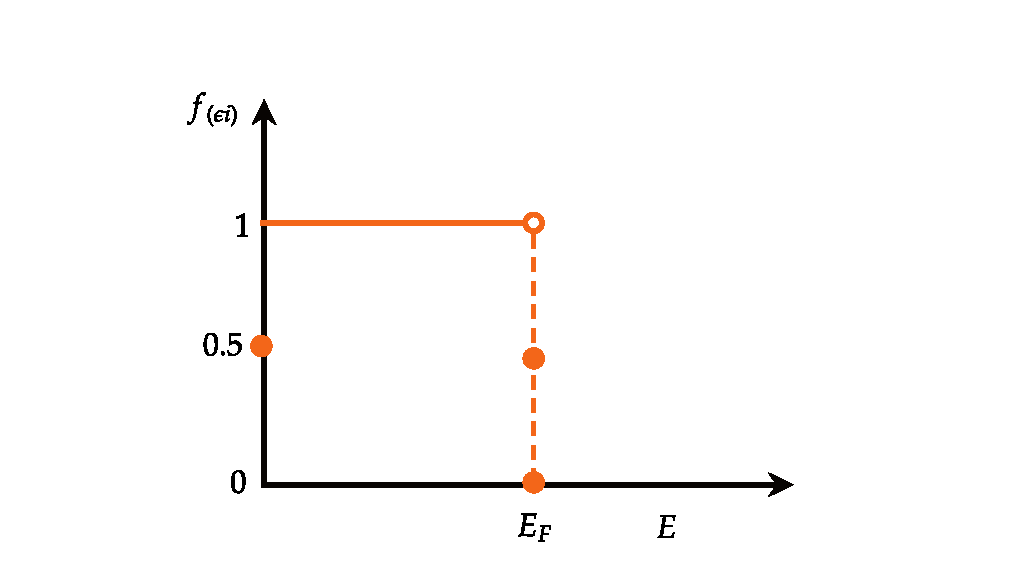
\includegraphics[height=5.5cm,width=9cm]{SM-II-01}
\end{figure}
\subsection{Fermi level at $T \neq 0 k$}
As temparature increases, the states below $E_{F}, f(\varepsilon)$ start decreasing and above $E_{F}$ Starts filling.
\begin{figure}[H]
	\centering
	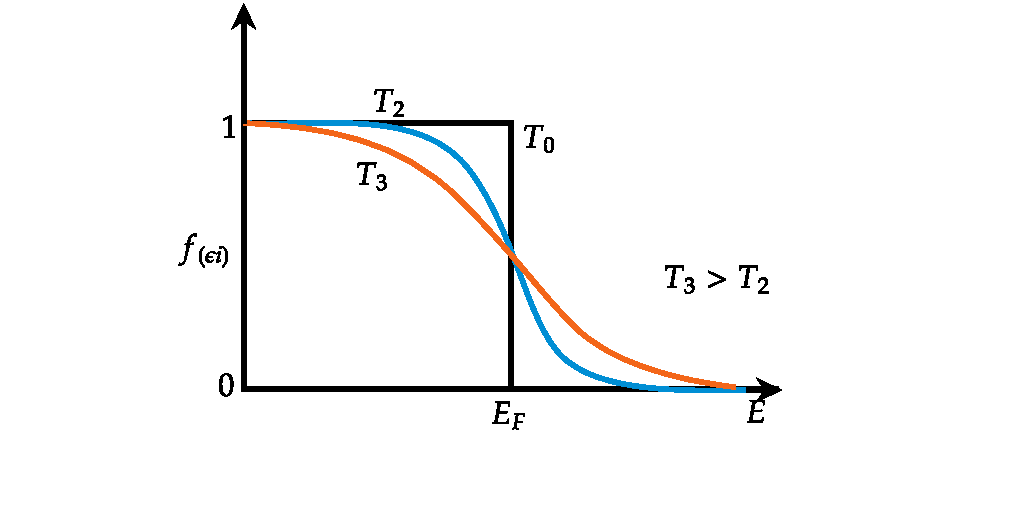
\includegraphics[height=5.5cm,width=9cm]{SM-II-02}
\end{figure}
\subsection{Fermi Wave Vector($K_f$)}
\begin{itemize}
	\item In 1-D : $K_{f}=\frac{N \pi}{2 L}$
	\item  In 2-D : $K_{f}=\left(\frac{2 \pi N}{Are a}\right)^{1 / 2}$
	\item  In 3-D : $k_{f}=\left(\frac{3 \pi^{2} N}{\text { Volume }}\right)^{1 / 3}$
\end{itemize}
Fermi Energy $E_{F}=\frac{\hbar^{2} k_{F}^{2}}{2 m}$\\
\renewcommand*{\arraystretch}{2}
\begin{tabular}{|p{4cm}|p{4cm}|p{3cm}|}
	\hline
	Fermi Energy&Zero Point Energy (Average Energy)&Dimension\\\hline
	$\frac{\hbar^{2}}{2 m}\left(3 \pi^{2} \rho\right)^{2 / 3}$&$\frac{3}{5} E_{F}$&3\\
	$\frac{\hbar^{2}}{2 m}(2 \pi \rho)$&$\frac{1}{2} E_{F}$&2\\
	$\frac{\hbar^{2}}{2 m}\left(\frac{N \pi}{2 L}\right)^{2}$&$\frac{1}{3} E_{F}$& 1\\\hline
\end{tabular}\\\\
Here $\mathrm{S}=$number density $\left(\frac{N}{V}\right.$ for $3 D ,\ \frac{N}{A}$ for $\left.2 D\right)$
\section{Grand Canonical Ensemble}
Grand canonical ensemble - An ensemble in which system can exchange both energy as well as particles with each other or particle energy reservoir.\\
Equilibrium - between a system and a particle energy reservoir :
We consider the given system A as immersed in a large reservoir A with which it can exchange both energy as well as particles. After some time both attain the state of mutual equilibrium. In equilibrium both have the same value of $\mathrm{T}$ and $\mu$, the number of particle and energy become variable whose values can vary at any time $\mathrm{t}$ any where between 0 to $\infty$. 

$P(\Omega, N_{\Omega)} \rightarrow$ probablity to find the system at a microstate $\Omega$, when total number of particles is $N_{\Omega}$, remember here total number of particle is not constant.
\begin{align*}
P\left(\Omega, N_{\Omega}\right)&=\frac{e^{-\beta\left[H\left(\Omega\right)-\mu N _\Omega\right]}}{Z(\mu, \Omega, T)}\\
H(\Omega) \rightarrow &\text { Hamiltonian }\\
\mu N_{\Omega} \rightarrow &\text { Chemical work }
\intertext{Grand canonical partition function }
\end{align*}
\begin{align*}
Z(M,\Omega,T)&=\sum_{\Omega,N_\Omega}\beta[H(\ \Omega)-N_{\Omega}M]\\
&=\sum_{N_\Omega=O}e^{\beta{\mu} N_{\Omega}}\sum e^{-\beta H(\Omega)}\\
&=\sum_{N_\Omega=O}e^{\beta{\mu} N_{\Omega}}Z\\
Z\rightarrow &\text{canonical partion function}\\
\sum_{N_\Omega=O} e^{\beta{\mu} N_{\Omega}}
\rightarrow&\text{ Fugacity}\\
\text{Grand Canonical Ensemble }&=\text{Fugacity}\times{Z_{canonical}}
\end{align*}
\textbf{Some Important relations connecting Grand Canonical Ensemble}
\begin{enumerate}
	\item Average number of particles $<N_\Omega>$=$\frac{1}{\beta}\frac{\partial}{\partial\mu}$$\ell n$Z\\
	\item Variance,$<N^{2}>$$\approx$N\\
	\item Standard deviation$<{N}^{2}>^{1/2}$$\approx$$N^{1/2}$\\
	\item $\frac{N^{1/2}}{<N>}\approx$$\frac{1}{N^{1/2}}$
\end{enumerate}
As $N\rightarrow \infty$, Grand canonical ensenble equivalent to microcanonical ensemble.
\section{Bose GAS}
Distribution function for Bose-Eienstien statistiss,
\begin{align*}
f(\varepsilon)&=\frac{1}{e^{\beta(\varepsilon_i-\mu)}-1}\\
&O\leq f(\varepsilon_i)\leq1\\
f(\varepsilon)\text{cannot}&\text{ be negative}\\
\therefore\quad&e^{\beta(\varepsilon_i-\mu)}>1\\
\text{Applying }&\text{logarithm.}\\
&\beta(\varepsilon_i-\mu)>0\\
&(\varepsilon_i-\mu)>0\\
\text{for ground state},\varepsilon_{i}&=0\\
\mu&=-ve\\
\text{for some bosons}&\text{ chemical potential is negative} \\
\text{for photons and phonons,}&\mu=0\\
\mu&=0\text{ or }-ve\text{ in Bose Particles.}
\end{align*}
\subsection{Bose Einstein Condensation(v state of matter)}
Rapid increas in the population of ground state,
when temparature is lowered below critical temparature is known sa Bose Eienstien Condenstion.That particular critical temparature is known as Bose temparature,$T_{B}.$\\
$N=N_{O}+Ne$\\
\begin{enumerate}
	\item At $T=T_{B}$
	\begin{align*}
	\intertext{	Condensation process is about to start at $T=T_{B}$It is like a tipping point and maximum number of particles are still in the exited state.}
	N&=N_{0}+N_{e},\text{ here $N_{0}$ is negligible}\\
	&N \approx N e.
	\end{align*}
	
	\textbf{Important points}
	\begin{align*}
	T_{B}&=\left(\frac{N}{V}\right)^{2 / 3} \frac{h^{2}}{(2 \cdot 612)^{2 / 3} \times 2 \pi m k g_{s}}\\
	g_{s} &\rightarrow\text{ degeneracy.}\\
	\frac{N}{V} &\rightarrow\text{ number density $=\rho$}\\
	T_{B} &\propto(\rho)^{2 / 3}\\
	T_{\beta} &\propto \frac{1}{m}
	\end{align*}
	
	\textbf{Genaral case}\\
	If $E \propto p^{s}$ \\$T_{B} \propto(\rho)^{s / d}$\\
	$d \rightarrow$ dimension.
	\item  $\quad T<T_{B}$\\
	Rapid increase in population of ground State when $T<T_{B}$.\\
	\textbf{Important points}\\
\end{enumerate}
\begin{align*}
&N=N_{0}+N_{e} \\
&N_{e}=N\left(\frac{T}{T_{\beta}}\right)^{3 / 2} \\
&N_{0}=N\left(1-\left(\frac{T}{T_{B}}\right)^{3 / 2}\right)
\end{align*}
\subsection	{Depandancy, of Various Thermodynamic variables on temparature'T'}
$\Rightarrow$ Relations are applicable to both FermiDirac 8 Bose Eienstien statistics.\\
$\Rightarrow$\textbf{ Important types of Systems }in frequently asking Questions.\\
\begin{enumerate}
	\item \textbf{Bose Eienstien statistics}\\
	Black body radiation\\
	Photon gas\\
	Any Bosonic system.\\
	\item\textbf{ Fermi-dirac statistics}\\
	Free electron gas\\
	White dwarf
\end{enumerate}
\subsection{Important relations}
\begin{enumerate}
	\item Total number of particles, $N^{\prime} \alpha T^{d / S}$\\
	\item$V\  \propto\  \frac{1}{T^{d/s-1}}$ \\
	\item\  $E \ \propto \ T^{d / s+1}$\\
	\item\  $C_{v} \ \propto\  T^{d / s}$\\
	\item $S \ \propto\  T^{d / s}$	
\end{enumerate}
\newpage
\begin{abox}
	Practise set-3
\end{abox}
\begin{enumerate}
	\item If the Partition function of a harmonic oscillator with frequency $w$ at a temperature $T$ is $k T/ \hbar w$, then the free energy of $N$ such independent oscillators is:
		\begin{tasks}(2)
			\task[\textbf{a.}]$\frac{3}{2} N K T$
			\task[\textbf{b.}]$k+\ln \frac{\hbar \omega}{k+}$
			\task[\textbf{c.}]NKT $\ln \frac{\mathrm{ke}}{\mathrm{KT}}$
			\task[\textbf{d.}] NKe $\ln \frac{\text { the }}{2 K T}$
		\end{tasks}
	\begin{answer}
		\begin{align*}
		z_{N} &=\left(\frac{K T}{\hbar \omega}\right)^{N} \\
		\langle A\rangle &=-K T \ln z_{N} \\
		&=-K T \ln \left(\frac{K T}{\hbar \omega}\right)^{N} \\
		&=N K+\ln \left(\frac{\hbar \omega}{K T}\right)
		\end{align*}
		So the correct answer is \textbf{Option(c)}
	\end{answer}
\item For a system of independent non-interacting 1-dimemtional oscillators, the valul of the free energy per oscillator, in the limit $T \rightarrow 0$ is:
	\begin{tasks}(2)
		\task[\textbf{a.}] $\frac{1}{2} \hbar \omega$
		\task[\textbf{b.}]$\hbar\omega$
		\task[\textbf{c.}]$\frac{3}{2} \hbar \omega$
		\task[\textbf{d.}] 0
	\end{tasks}
\begin{answer}
	\begin{align*}
	z_{N}&=\left[2 \sinh \left(\frac{\beta \hbar \omega l}{2}\right)\right]^{-N}\\
	U&=\frac{\hbar \omega}{2} N \cot h\left(\frac{\beta \hbar u}{2}\right)\\
	\text { as } T \rightarrow 0 &\Rightarrow \beta \rightarrow \infty\\
	U&=\frac{N \hbar \omega}{2} \Rightarrow \frac{U}{N}=\frac{1}{2} \hbar \omega\\
	F&=U-T S=U \text { as } T=0\\
	F&=U\\
	\frac{F}{N}&=\frac{1}{2} \hbar \omega
	\end{align*}
	So the correct answer is \textbf{Option(a)}
\end{answer}	
\item For a quantum mechanical Harmonic oscillator with energy $E_{n}=\left(n+\frac{1}{2}\right) \hbar \omega$. The Partition $f x^{n}$ is:
\begin{tasks}(2)
	\task[\textbf{a.}]$\frac{e^{\hbar\omega/K_BT}}{e^{\hbar\omega/K_BT}-1}$
	\task[\textbf{b.}]$e^{\hbar \omega / 2 K_{B} T}-1$
	\task[\textbf{c.}]$e^{\hbar  \omega / 2 K_{B} T}-1$
	\task[\textbf{d.}] $\frac{e^{\hbar\omega/K_BT}}{e^{\hbar\omega/2K_BT}-1}$
\end{tasks}
\begin{answer}
	\begin{align*}
	E_{n}&=\left(n+\frac{1}{Q}\right) \text { tue } \rightarrow 1 \rightarrow \operatorname{Dim} \text { Q.H.0 }\\
	z_{1}&=\sum_{n} e^{\beta E}\\
	z_1&=e^{-\beta\left(n+\frac{1}{2} \right) }\hbar \omega\\
	z&=e^{-\beta \hbar \omega / 2}\left[1+e^{-\beta \hbar \omega}+e^{-2 \beta \hbar \omega}+\right]\\
	z_{1}&=\frac{e^{-\beta \hbar \omega / 2}}{1-e^{-\beta \hbar \omega}}=\left[2 \sinh \left(\frac{\beta \hbar \omega}{2}\right)\right]^{-1}\\
	z_{1}&=\frac{e^{-\beta \hbar \omega \mid \alpha}}{1-e^{-\beta \hbar \omega}} \times \frac{e^{\beta \hbar \omega}}{e^{\beta \hbar \omega}}\\
	z_{1}&=\frac{e^{\beta \hbar \omega / 2}}{e^{\beta \hbar \omega}-1}\hspace{1cm} \beta=\frac{1}{K T}\\
	z_{1}&=\frac{e^{\hbar \omega / 2 K_{B} T}}{e^{\hbar \omega / K_{B} T}-1}
	\end{align*}
	So the correct answer is \textbf{Option(d)}
\end{answer}
\item 	The probability of a system to be in a state with energy E at temperature T is proportional to $e^{-E \mid K_{B} T}$. If the system in question is a 1-Dim. quantum H.O of frequency $\omega$ the average energy at temperature T is
	\begin{tasks}(2)
		\task[\textbf{a.}]$\frac{\hbar\omega}{2}$
		\task[\textbf{b.}]$\hbar \omega\left(e^{-\hbar \omega K_{B} T}+\frac{1}{2}\right)$
		\task[\textbf{c.}]$\hbar \omega\left(\frac{1}{e^{\hbar\omega/KT_{-1}}}+\frac{1}{2}\right)$
		\task[\textbf{d.}] $\hbar \omega\left(\frac{1}{e^{\hbar\omega/KT_{+1}}}+\frac{1}{2}\right)$
	\end{tasks}
\begin{answer}
	\begin{align*}
	\intertext{for $1-Dim Q \cdot H \cdot 0$ :}
	z_{1}&=\frac{e^{-\beta \hbar \omega / 2}}{1-e^{-\beta \hbar \omega}}\\
	u&=-\frac{\partial}{\partial \beta} \ln z_{1}=-\frac{\partial}{\partial \beta}\left[-\frac{\beta \hbar \omega}{2}-\ln \left(1-e^{-\beta \hbar \omega}\right)\right.\\
	v&=\frac{\hbar \omega}{2}+\frac{e^{-\beta \hbar u}}{1+\left(-e^{-\beta \hbar u e}\right)} \hbar \omega\\
	u&=\hbar \omega\left(\frac{e^{-\beta \hbar \omega}}{1-e^{-\beta \hbar \omega}+\frac{1}{2}}\right)\\
	\text { also } v&=\frac{\hbar \omega}{2} \cot h\left(\frac{\beta \hbar \omega}{2}\right)
	\end{align*}
	So the correct answer is \textbf{Option(c)}
\end{answer}	
\item A system has two normal modes of vibration, with frequencies $\omega_{1}\text{ and }\omega_{2}=2\omega_{1}$. What is the probability that at temperature $T$, the system has an energy less than $\mu\hbar\omega_{1}$? (use $x=e^{\beta \hbar \omega}$ and $z$ is as partition $fx^n$)
	\begin{tasks}(2)
		\task[\textbf{a.}]$x^{3 / 2}\left(x+2 x^{2}\right) / 2$
		\task[\textbf{b.}]$x^{3 / 2}\left(1+x+x^{2}\right) / 2$
		\task[\textbf{c.}] $x^{3 / 2}\left(1+2 x^{2}\right) / 2$
		\task[\textbf{d.}] $x^{3 / 2}\left(1+x+2 x^{2}\right) / 2$
	\end{tasks}
\begin{answer}
	\begin{align*}
	E&=\left(n+\frac{1}{2}\right) \hbar u_{1}+\left(n+\frac{1}{2}\right) \hbar\left(2 v_{1}\right)\\
	E&=\left(3 n+\frac{3}{2}\right) \text { hul }\\
	E_{0,0}&=\frac{3}{2} \hbar u_{1} ; E_{1,0}=\frac{5}{2} \hbar \omega_{1}; \quad E_{2}=\frac{7}{2} \hbar u_{1}\\
	P_{i}&=\frac{g_{i} e^{-\beta \varepsilon_{i}}}{2}\hspace{3cm}\left(\begin{array}{ll}
	n_{2}=0, & n_{1}=2 \\
	n_{2}=1, & n_{1}=0
	\end{array}\right)\\
	P_{i}&=\left(e^{-3 / 2 \beta t \omega e}+e^{-\frac{5}{2} \beta \hbar \omega}+2 e^{-\frac{7}{2} \beta \hbar \omega}\right) \mid 2\\
	\text { Put } x&=e^{-\beta \hbar \omega}\\
	P_{i}&=\frac{x^{3 / 2}+x^{5 / 2}+2 x^{7 / 2}}{2}=\frac{x^{3 / 2}\left(1+x+2 x^{2}\right)}{2}
	\end{align*}
	So the correct answer is \textbf{Option(d)}
\end{answer}
	\item Spin $\frac{1}{2}$ ions of magnetic moment $H$ each is kept in an external magnetic field $H$. If the system is in equilibrium at temperature $T$, then Helmholtz free energy of the system is 
		\begin{tasks}(2)
			\task[\textbf{a.}]$N K_{B} T \ln \left(\cosh \frac{H H}{K_{B} T}\right)$
			\task[\textbf{b.}]$-N K_{B} T \ln \left(2 \cosh \frac{4 H}{K_{B} T}\right)$
			\task[\textbf{c.}]$N K_{B} T \ln \left(2 \cosh \frac{H H}{K_{B} T}\right)$
			\task[\textbf{d.}] $-N K_{B} T \ln \left(2 \sin R \frac{\mu H}{K_{B} T}\right)$
		\end{tasks}
	\begin{answer}
		\begin{align*}
		z&=e^{\beta \varepsilon}+e^{-\beta \varepsilon}\\
		z&=2 \cosh \beta \varepsilon=2 \cosh \left(\frac{\mu H}{K_{B} T}\right)\\
		Z_{N}&=\left[2 \cos h\left(\frac{4 H}{K_{B} T}\right)\right]^{N}\\
		\langle A\rangle&=-k T \ln z_{N}\\
		\langle A\rangle&=-k T \ln \left(2 \cosh \frac{M n}{K_{B} T}\right)^{N}\\
		\langle A\rangle&=-N K T \ln \left(2 \cosh \frac{\mu H}{K_{B} T}\right)
		\end{align*}
		So the correct answer is \textbf{Option(b)}
	\end{answer}
\item Consider a system of $N$ non-interacting spin $\frac{1}{2}$ particles, each having a magnetic moment $H$ is in a magnetic field $\vec{B}=B \hat{z} $. If $E$ is the total energy then number of accessible microstates $\Omega$ is.
\begin{tasks}(2)
	\task[\textbf{a.}]$R=\frac{N !}{\frac{1}{Q}\left(N-\frac{E}{H B}\right) ! \frac{1}{Q}\left(N+\frac{E}{H B}\right) !}$
	\task[\textbf{b.}]$\Omega=\frac{\left(N-\frac{E}{H B}\right) !}{\left(N+\frac{E}{H B}\right) !}$
	\task[\textbf{c.}]$R=\frac{1}{2}\left(N-\frac{E}{H B}\right) ! \frac{1}{2}\left(N+\frac{E}{H B}\right) !$
	\task[\textbf{d.}] $\Omega=\frac{N !}{\left.N+\frac{E}{H B}\right) !}$
\end{tasks}
\begin{answer}
	\begin{align*}
	M&=N_{1}+N_{2}\\
	E&=-N_{1} H B+N_{2} H B \Rightarrow \frac{E}{H B}=-N_{1}+N_{2}\\
	N_{2}&=\frac{1}{2}\left[N+\frac{E}{\mu B}\right] \quad 4 N_{1}=\frac{1}{2}\left[N-\frac{E}{\mu B}\right]\\
	\Omega&=\frac{N !}{\frac{1}{2}\left(N-\frac{E}{H B}\right) ! \frac{1}{2}\left(N+\frac{E}{M B}\right) !}
	\end{align*}
	So the correct answer is \textbf{Option(a)}
\end{answer}	
	
	
	
	
	
	
	
	
	
	
	
	
	
	
\end{enumerate}